\chapter{Oszillator-Wellenfunktionen, Spin-einhalb und Teilchenaustausch}

\section{Oszillatoren überall}

Jedes System mit einem stabilen Gleichgewicht kann schwingen, wenn es aus diesem Gleichgewicht ausgelenkt wird. Es kann eine oder mehrere Frequenzen haben. Eine Violinsaite besitzt zum Beispiel eine Grundschwingung und höhere Harmonische. Zupft man sie an, wird eine bestimmte Kombination dieser Schwingungsmoden angeregt.

Die wichtigeren Beispiele hier sind Felder. Die Gleichgewichtskonfiguration des elektromagnetischen Feldes ist das Vakuum: kein elektrisches Feld, kein magnetisches Feld und keine elektromagnetische Schwingung. Strahlt man in einen Hohlraum oder einen Wellenleiter ein, kann das Feld in seinen erlaubten Moden schwingen, jede mit ihrer eigenen Frequenz. In der Quantentheorie beschreiben diese Moden Ansammlungen von Photonen.

Dieselbe Idee gilt für einen Kristall. Es wäre irreführend, sich jedes Atom als unabhängigen Oszillator vorzustellen. Die Atome üben Kräfte aufeinander aus, sodass die Auslenkung eines Atoms seine Nachbarn beeinflusst und eine Welle durch den Kristall läuft. Die Normalmoden dieser gekoppelten Bewegung sind harmonische Oszillatoren; ihre Quanten heißen Phononen. Photonen und Phononen sind unterschiedliche physikalische Objekte, führen aber beide zurück zur selben Oszillatoralgebra.

\section{Die Oszillatoralgebra}

Für die Betrachtung des Oszillators setzen wir Masse und reduziertes Plancksches Wirkungsquantum gleich eins:
\[
m=1,\qquad \hbar=1.
\]
Der Hamiltonoperator lautet
\begin{equation}
H=\frac{p^{2}}{2}+\frac{\omega^{2}x^{2}}{2}.
\end{equation}
Der Parameter \(\omega\) legt die Krümmung des Potentials fest und ist zugleich die Schwingungsfrequenz.

Wir definieren die Auf- und Absteigeoperatoren durch
\begin{equation}
A_{\pm}=\frac{p\pm i\omega x}{\sqrt{2\omega}}.
\end{equation}
Die Normierung ist so gewählt, dass
\begin{equation}
[A_{-},A_{+}]=1.
\end{equation}
Der Zahloperator ist
\begin{equation}
N=A_{+}A_{-}.
\end{equation}
Zusammen bedeuten diese Gleichungen, dass \(A_{+}\) einen Eigenwert von \(N\) um eins erhöht und \(A_{-}\) ihn um eins erniedrigt. Das resultierende Spektrum lautet
\begin{equation}
n=0,1,2,3,\ldots .
\end{equation}

Das Produkt der beiden Leiteroperatoren macht auch die quantenmechanische Korrektur der klassischen Energie sichtbar:
\begin{align}
N
&=\frac{1}{2\omega}(p+i\omega x)(p-i\omega x)\\
&=\frac{1}{2\omega}\left(p^{2}+\omega^{2}x^{2}
 +i\omega[x,p]\right)\\
&=\frac{1}{2\omega}\left(p^{2}+\omega^{2}x^{2}-\omega\right),
\end{align}
wobei \([x,p]=i\) gilt. Folglich ist
\begin{equation}
H=\omega\left(N+\frac12\right).
\end{equation}
Ist die additive Konstante für das Problem unerheblich, verwendet man zweckmäßig den verschobenen Hamiltonoperator
\begin{equation}
H_{\mathrm{shifted}}=H-\frac{\omega}{2}=\omega N.
\end{equation}
Der Term \(\omega/2\) ist die Nullpunktsenergie oder Grundzustandsenergie des Oszillators. Bei einer Feldmode heißt der entsprechende Term Vakuumenergie. Er spiegelt die Unschärferelation wider: Kein Zustand kann zugleich \(x\) und \(p\) exakt gleich null haben; daher können die beiden positiven quadratischen Terme in \(H\) nicht beide den Erwartungswert null haben.

\begin{classroomqa}
\lecturetimestamp{00:09:46}
\audiencequestion{Warum gehört null zum Spektrum des Zahloperators?}
\lecturerresponse{Das lässt sich explizit zeigen, indem man die Wellenfunktion des Grundzustands konstruiert. Dabei wird ein Zustand mit \(N=0\) sichtbar.}
\end{classroomqa}

Beginnen wir diese Konstruktion, indem wir Zustandsvektoren durch Ortswellenfunktionen ersetzen. Die Energieeigenzustände werden zu
\[
\psi_{0}(x),\ \psi_{1}(x),\ \psi_{2}(x),\ldots,
\]
und die Grundoperatoren wirken als
\begin{equation}
X\longmapsto x,\qquad
P\longmapsto -i\frac{d}{dx}.
\end{equation}
Stellt man \(\hbar\) wieder her, lautet die zweite Ersetzung
\(P\mapsto-i\hbar\,d/dx\).

Bevor wir \(\psi_{0}\) bestimmen, gibt es eine schnellere, abstrakte Antwort auf die Frage. Auf der diskreten Leiter der normierbaren Oszillatoreigenzustände ist \(N=A_{+}A_{-}\) nichtnegativ; wiederholtes Absteigen in Einerschritten kann daher nicht unbegrenzt weitergehen. Am Endpunkt---dessen normierbare Wellenfunktion wir unten konstruieren---muss es einen Zustand geben, bezeichnet mit \(\lvert0\rangle\), für den gilt:
\begin{equation}
A_{-}\lvert0\rangle=\mathbf 0.
\end{equation}
Andernfalls wäre \(A_{-}\lvert0\rangle\) ein weiterer Zustand eine Stufe tiefer. Daraus folgt unmittelbar
\begin{equation}
N\lvert0\rangle
=A_{+}A_{-}\lvert0\rangle
=\mathbf 0
=0\,\lvert0\rangle.
\end{equation}
Der unterste Zustand hat also den Zahleneigenwert null.

\begin{classroomqa}
\lecturetimestamp{00:14:57}
\audiencequestion{Wenn null der Eigenwert ist, müsste dann auf der rechten Seite ein Eigenvektor zum Eigenwert null stehen?}
\lecturerresponse{Das Ket \(\lvert0\rangle\) ist ein normierter, von null verschiedener Vektor mit der Bezeichnung null. In \(N\lvert0\rangle=0\,\lvert0\rangle\) ist die rechte Seite der Nullvektor. Das Ket des Grundzustands und der Nullvektor sind verschiedene Objekte.}
\end{classroomqa}

\section{Die Schr\"odinger-Gleichung und physikalische Lösungen}

Kehren wir nun zur Ortsdarstellung zurück. Die zeitunabhängige Schr\"odinger-Gleichung lautet
\begin{equation}
\left[
-\frac12\frac{d^{2}}{dx^{2}}
+\frac12\omega^{2}x^{2}
\right]\psi(x)=E\psi(x).
\end{equation}
Als Differentialgleichung zweiter Ordnung besitzt sie formale Lösungen für beliebige Werte von \(E\). Die meisten dieser formalen Lösungen sind keine physikalischen Osillatorzustände. Für große \(\lvert x\rvert\) wachsen sie exponentiell, sodass ihre Norm divergiert.

Für einen gebundenen Zustand muss die Wellenfunktion quadratintegrabel sein:
\begin{equation}
\int_{-\infty}^{\infty}\psi^{*}(x)\psi(x)\,dx<\infty.
\end{equation}
Dann kann sie so normiert werden, dass das Integral eins ergibt. Nur bestimmte Energiewerte liefern solche Lösungen. Orts- und Impulszustände auf einer unendlichen Geraden sind diesbezüglich Ausnahmefälle; exponentiell anwachsende Oszillatorlösungen werden dagegen einfach aus dem Zustandsraum ausgeschlossen.

\section{Der gaußförmige Grundzustand}

Die Differentialgleichung zweiter Ordnung lässt sich lösen, doch die Leiteralgebra liefert eine einfachere Gleichung erster Ordnung:
\begin{equation}
A_{-}\psi_{0}(x)=0.
\end{equation}
Der Vorfaktor in \(A_{-}\) ist unerheblich, wenn die rechte Seite null ist; dies ist daher äquivalent zu
\begin{equation}
(p-i\omega x)\psi_{0}(x)=0.
\end{equation}
Mit \(p=-i\,d/dx\) ergibt sich
\begin{equation}
\left(\frac{d}{dx}+\omega x\right)\psi_{0}(x)=0.
\end{equation}

\begin{classroomqa}
\lecturetimestamp{00:22:32}
\audiencequestion{Lässt sich das durch Trennung der Variablen lösen?}
\lecturerresponse{Es gibt nur eine unabhängige Variable, also keine zwei Variablen, die man trennen könnte. In der Form \(\psi_{0}'/\psi_{0}=-\omega x\) hat die Gleichung die Gestalt einer logarithmischen Ableitung. Das legt nahe, die Wellenfunktion als Exponentialfunktion anzusetzen.}
\end{classroomqa}

Eine nützliche Lösungsmethode besteht darin, anzusetzen:
\begin{equation}
\psi_{0}(x)=e^{f(x)}.
\end{equation}
Dann gilt
\[
\psi_{0}'(x)=f'(x)e^{f(x)},
\]
und der gemeinsame Exponentialfaktor kürzt sich heraus. Die Gleichung vereinfacht sich zu
\begin{equation}
\frac{df}{dx}+\omega x=0.
\end{equation}

\begin{classroomqa}
\lecturetimestamp{00:26:28}
\audiencequestion{Müsste in \(f(x)\) ein Minuszeichen stehen?}
\lecturerresponse{Ja. Da \(df/dx=-\omega x\) gilt, ergibt die Integration einen negativen quadratischen Term.}
\end{classroomqa}

Somit gilt
\begin{equation}
f(x)=-\frac12\omega x^{2}+C,
\end{equation}
und
\begin{equation}
\psi_{0}(x)\propto e^{-\omega x^{2}/2}.
\end{equation}
Die multiplikative Normierungskonstante bleibt unbestimmt. Entscheidend ist die gaußförmige Gestalt: Die Wellenfunktion ist glatt, um den Ursprung konzentriert und fällt für große \(\lvert x\rvert\) rasch ab. Sie ist offensichtlich quadratintegrabel.

Man muss die Lösung nicht in die Differentialgleichung zweiter Ordnung einsetzen, um ihre Energie zu bestimmen. Die Algebra liefert bereits
\begin{equation}
E_{0}=\frac{\omega}{2}.
\end{equation}

\section{Angeregte Zustände, Knoten und klassische Bewegung}

Der erste angeregte Zustand ergibt sich, indem man auf den Grundzustand den Aufsteigeoperator anwendet:
\begin{equation}
\psi_{1}(x)\propto A_{+}\psi_{0}(x)
\propto(p+i\omega x)e^{-\omega x^{2}/2}.
\end{equation}
Die Grundzustandsgleichung besagt
\[
p\psi_{0}=i\omega x\,\psi_{0}.
\]
Durch das Vorzeichenwechseln im Leiteroperator wird aus der Auslöschung eine Addition:
\begin{equation}
(p+i\omega x)\psi_{0}
=2i\omega x\,\psi_{0}.
\end{equation}
Bis auf einen Gesamtfaktor gilt
\begin{equation}
\psi_{1}(x)\propto x\,e^{-\omega x^{2}/2}.
\end{equation}

Diese Wellenfunktion ist ungerade:
\begin{equation}
\psi_{1}(-x)=-\psi_{1}(x).
\end{equation}
Ihre Wahrscheinlichkeitsdichte ist gerade, hat aber am Ursprung einen Knoten:
\begin{equation}
\lvert\psi_{1}(0)\rvert^{2}=0.
\end{equation}
Die Wahrscheinlichkeitsdichte des ersten angeregten Zustands hat also bei \(x=0\) einen Knoten.

Wiederholte Anwendung von \(A_{+}\) liefert Polynome höheren Grades, die mit derselben gaußförmigen Einhüllenden multipliziert sind.\footnote{Die Vorlesung nennt die Polynomfaktoren höheren Grades, den bei jedem Schritt hinzukommenden Knoten und den Symmetriewechsel von \(00{:}34{:}25\) bis \(00{:}35{:}49\). Die Form als Produkt aus Gaußfunktion und Polynom wird durch Leonard Susskind und Art Friedman, \emph{Quantum Mechanics: The Theoretical Minimum} (2014), in ihrer Behandlung der Oszillatoreigenfunktionen bestätigt.} Bis auf einen Normierungsfaktor gilt
\begin{equation}
\psi_{n}(x)=P_{n}(x)e^{-\omega x^{2}/2}.
\end{equation}
Die Parität wechselt zwischen gerade und ungerade, und bei jedem Schritt kommt ein Knoten hinzu. Mit wachsendem \(n\) breitet sich die Wellenfunktion weiter vom Ursprung aus und weist raschere Oszillationen auf.

Diese beiden Eigenschaften haben direkte physikalische Bedeutungen. Eine größere Ausdehnung vom Ursprung entspricht einer höheren potenziellen Energie, weil das Potential wie \(x^{2}\) anwächst. Rasche Oszillationen im Ortsraum signalisieren einen größeren Impuls. Ein stark angeregter Oszillator gelangt wahrscheinlich weiter vom Zentrum weg; beim Durchgang durch den Zentralbereich trägt er mehr Impuls, und seine Wellenfunktion oszilliert dort rascher.

\begin{classroomqa}
\lecturetimestamp{00:37:18}
\audiencequestion{Nähert sich der harmonische Oszillator keinem klassischen Verhalten an, wenn \(n\) groß wird?}
\lecturerresponse{Klassische Bewegung wird nicht durch einen einzigen stationären Energieeigenzustand beschrieben. Sie zeigt sich in einem Wellenpaket, das viele Energieniveaus enthält. Eine verschobene Gaußfunktion entwickelt sich beispielsweise wie ein klassischer Oszillator hin und her, und die relative Unschärfe wird kleiner, je größer die Schwingungsamplitude ist.}
\end{classroomqa}

Beginnen wir mit der gaußförmigen Wellenfunktion des Grundzustands und verschieben sie vom Ursprung weg. Das verschobene Wellenpaket ist kein Energieeigenzustand mehr, sondern eine Überlagerung vieler solcher Zustände. Unter der zeitabhängigen Schr\"odinger-Gleichung sammeln seine Komponenten unterschiedliche Phasen an. Das Paket schwingt von einer Seite des Potentials zur anderen, wobei es nahe dem Zentrum eine rasche Phasenvariation entwickelt und an einem Umkehrpunkt wieder glatt wird. Je größer die Auslenkung im Verhältnis zur Breite des Pakets ist, desto klassischer erscheint die Bewegung.

\begin{classroomqa}
\lecturetimestamp{00:39:29}
\audiencequestion{Müsste die Wellenfunktion des zweiten angeregten Zustands am Ursprung null sein?}
\lecturerresponse{Nein. Ihr Polynomfaktor ist nicht einfach \(x^{2}\); er enthält auch einen konstanten Term, sodass die Wellenfunktion bei \(x=0\) nicht notwendigerweise verschwindet.}
\end{classroomqa}

Das Leiterargument setzt außerdem voraus, dass \(A_{+}\) und \(A_{-}\) auf dem quadratintegrablen Oszillatordomänenbereich hermitesch konjugiert sind und das für die Adjungiertheitsrelation erforderliche Randverhalten erfüllen. Exponentiell anwachsende formale Lösungen gehören nicht zu diesem Definitionsbereich.

\begin{classroomqa}
\lecturetimestamp{00:40:45}
\audiencequestion{Gibt es eine allgemeine Methode zu erkennen, ob sich ein Hamiltonoperator mit diesen algebraischen Methoden lösen lässt?}
\lecturerresponse{Eine solche allgemeine Regel gibt es nicht. Exakt lösbare Beispiele sind selten. Der harmonische Oszillator und das ideale nichtrelativistische Wasserstoffatom sind glückliche Fälle, in denen algebraische Methoden funktionieren.}
\end{classroomqa}

\section{Spin-einhalb als Drehimpuls}

Spin ist ein Drehimpuls, den ein Teilchen unabhängig von seiner Schwerpunktsbahbewegung trägt. Ein ruhendes Teilchen besitzt keinen Bahndrehimpuls \(\mathbf R\times\mathbf P\), kann aber dennoch Spin haben. Man kann versuchen, sich ein winziges rotierendes Objekt vorzustellen, oder Spin als intrinsische Quanteneigenschaft auffassen. Entscheidend ist die mathematische Aussage: Seine Komponenten transformieren sich unter räumlichen Drehungen und erfüllen die Kommutationsrelationen des Drehimpulses.

Von hier an stellen wir \(\hbar\) wieder her. Die Drehimpulskomponenten erfüllen
\begin{equation}
[L_{z},L_{x}]=i\hbar L_{y},
\end{equation}
wobei sich die beiden anderen Relationen durch zyklische Vertauschung ergeben. Die dimensionslosen Pauli-Matrizen sind
\begin{equation}
\begin{aligned}
\sigma_{z}&=
\begin{pmatrix}
1&0\\
0&-1
\end{pmatrix},\\[0.4em]
\sigma_{x}&=
\begin{pmatrix}
0&1\\
1&0
\end{pmatrix},\\[0.4em]
\sigma_{y}&=
\begin{pmatrix}
0&-i\\
i&0
\end{pmatrix}.
\end{aligned}
\end{equation}
In dieser Basis ist \(\sigma_{z}\) diagonal. Seine Eigenwerte sind \(+1\) und
\(-1\).

\begin{classroomqa}
\lecturetimestamp{00:47:35}
\audiencequestion{Müsste in \(\sigma_x\) ein Minuszeichen stehen?}
\lecturerresponse{Nein. Beide Nebendiagonalelemente von \(\sigma_x\) sind positiv.}
\end{classroomqa}

Die Tafelrechnung bei \(00{:}49{:}35\) beginnt mit der Multiplikation der einzelnen Matrixeinträge. Führt man die Produkte vollständig aus, erhält man
\begin{align}
\sigma_{z}\sigma_{x}
&=
\begin{pmatrix}
0&1\\
-1&0
\end{pmatrix}
=i\sigma_{y},\\
\sigma_{x}\sigma_{z}
&=
\begin{pmatrix}
0&-1\\
1&0
\end{pmatrix}
=-i\sigma_{y}.
\end{align}
Damit gilt
\begin{equation}
[\sigma_{z},\sigma_{x}]=2i\sigma_{y}.
\end{equation}
Der zusätzliche Faktor zwei entfällt, wenn man die physikalischen Spinoperatoren wie folgt definiert:\footnote{Bei der Tafelrechnung wird \(\hbar\) unterdrückt. Hier wird es wieder eingesetzt, damit \(S_i\) die Einheit eines Drehimpulses hat.}
\begin{equation}
S_{i}=\frac{\hbar}{2}\sigma_{i}.
\end{equation}
Dann gilt
\begin{equation}
[S_{z},S_{x}]=i\hbar S_{y},
\end{equation}
und entsprechend für zyklische Vertauschungen. Die Hälfte der Pauli-Matrizen bildet, mit wiederhergestelltem Faktor \(\hbar\), somit ein Drehimpulssystem.

Setzt man \(\hbar=1\), erhält man die unten gezeigte Form.\footnote{Das Quellbild ist \texttt{lecture\_04\_frame\_02.png}.}
\begin{figure}[htbp]
\centering
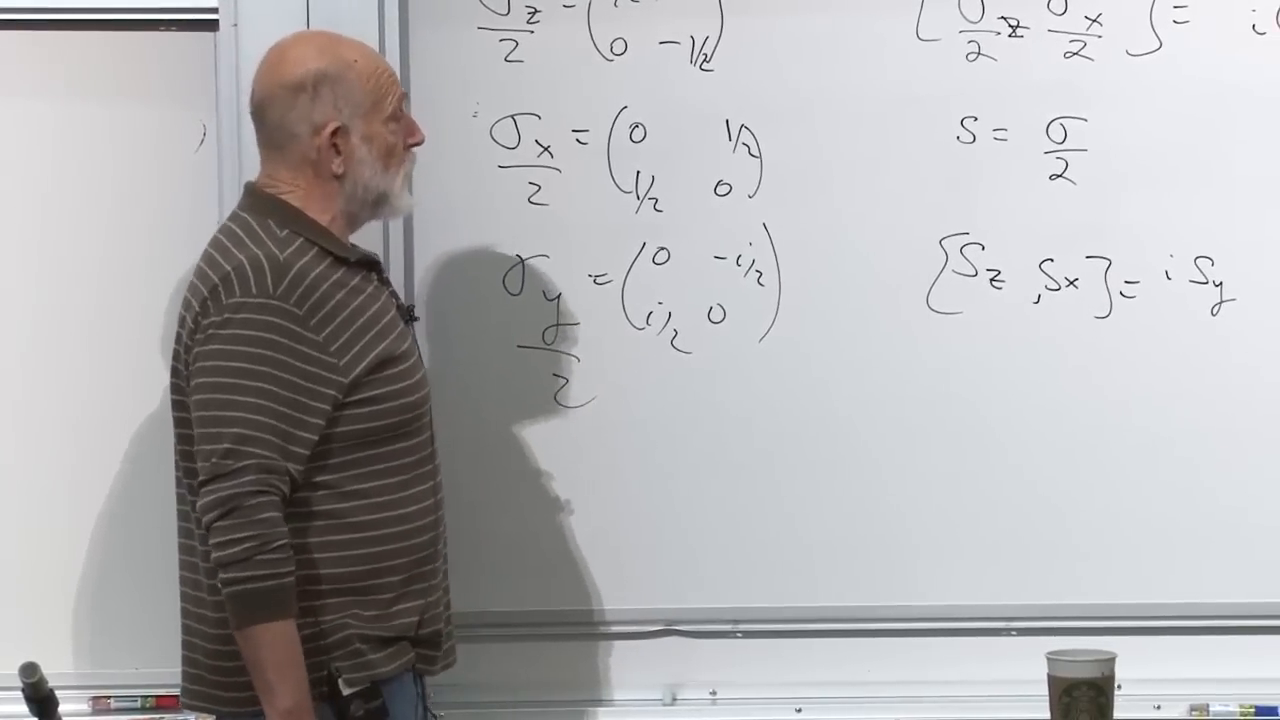
\includegraphics[width=0.9\linewidth]{lecture_04_frame_02.png}
\caption{In Einheiten, in denen \(\hbar=1\) gilt, sind die halben Pauli-Matrizen die Drehimpulsoperatoren für Spin einhalb und erfüllen \([S_z,S_x]=iS_y\).}
\lectureframe{00:55:41}
\end{figure}

Die beiden Eigenwertgleichungen für \(S_z\) lauten
\begin{equation}
S_z\lvert\pm\rangle
=\pm\frac{\hbar}{2}\lvert\pm\rangle.
\end{equation}
Äquivalent dazu ist die dimensionslose magnetische Quantenzahl
\begin{equation}
m_{s}=\pm\frac12,
\qquad
S_{z}\lvert m_{s}\rangle
=m_{s}\hbar\,\lvert m_{s}\rangle.
\end{equation}
Drehimpuls-Auf- und -Absteigeoperatoren verschieben \(m\) in ganzzahligen Schritten; daraus folgt jedoch nicht, dass jede Leiter durch null verlaufen muss. Multipletts mit ganzzahligem Drehimpuls enthalten ganzzahlige \(m\)-Werte, während Multipletts mit halbzahligen Drehimpulswerten halbzahlige Werte enthalten. Für Spin-einhalb umfasst die Leiter nur die beiden Zustände \(m_s=+1/2\) und \(m_s=-1/2\).

Diese beiden Zustände bilden das Spin-einhalb-Dublett. Elektronen, Myonen, Neutrinos und Quarks gehören zu den Teilchen, die durch solche Multipletts mit halbzahligem Spin beschrieben werden.

\section{Bahn- und Spin-Drehimpuls}

Es gibt nun zwei Arten von Drehimpuls. Der Bahndrehimpuls beschreibt die Bewegung relativ zu einem Ursprung:
\begin{equation}
\mathbf L=\mathbf R\times\mathbf P,
\end{equation}
\(\mathbf S\) ist dagegen intrinsischer Spin. Ihre Vektorsumme ist der Gesamtdrehimpuls:
\begin{equation}
\mathbf J=\mathbf L+\mathbf S.
\end{equation}

\begin{classroomqa}
\lecturetimestamp{00:56:49}
\audiencequestion{Wie lässt sich bei einem System mit dem Gesamtdrehimpuls \(\mathbf J\) sein Spin \(\mathbf S\) bestimmen?}
\lecturerresponse{Die Spin- und Bahndrehimpulsquantenzahlen werden gewöhnlich getrennt angegeben. Wenn \(L=0\) gilt, ist der gesamte Drehimpuls Spin. Andernfalls benötigt man die Quantisierungsregeln für die Addition von Drehimpulsen, die hier erst später behandelt werden.}
\end{classroomqa}

Die Additionsregeln gelten gleichermaßen für Bahndrehimpuls plus Spin, für zwei Spins oder für zwei Bahndrehimpulse. Das zusammengesetzte System besitzt eigene erlaubte Werte des Gesamtdrehimpulses; diese Regeln brauchen wir aber noch nicht.

\begin{classroomqa}
\lecturetimestamp{00:58:18}
\audiencequestion{Welche experimentellen Befunde führten zur Einführung des Spins?}
\lecturerresponse{Die Spektroskopie lieferte Hinweise, doch das Periodensystem bietet eine besonders anschauliche Motivation: Seine Schalenstruktur erfordert, dass Elektronen eine zusätzliche zweifach mögliche Eigenschaft besitzen.}
\end{classroomqa}

\section{Entartung des wasserstoffähnlichen Atoms und Schalenbesetzung}

Für den Bahndrehimpuls lautet die Eigenwertgleichung von \(L^{2}\)
\begin{equation}
L^{2}\lvert\ell,m\rangle
=\hbar^{2}\ell(\ell+1)\lvert\ell,m\rangle,
\end{equation}
Zu einem festen Wert von \(\ell\) gehören
\begin{equation}
2\ell+1
\end{equation}
magnetische Zustände, entsprechend \(m=-\ell,-\ell+1,\ldots,\ell\).

Das ideale nichtrelativistische Coulomb-Problem weist eine zusätzliche Entartung auf. Seine gebundenen Zustände haben negative Energien, die sich von unten null annähern; für die Zählung kommt es jedoch nur auf die Zuordnung der Niveaus zueinander an. Das erste Niveau mit \(\ell=1\) fällt mit dem nächsten Niveau mit \(\ell=0\) zusammen; das erste Niveau mit \(\ell=2\) kommt zur nächsten Hauptschale hinzu; und das Muster setzt sich fort.\footnote{\texttt{lecture\_04\_frame\_03.png}, \(01{:}02{:}01\); die vollständige Zuordnung der Hauptschalen wird von \(01{:}02{:}33\) bis \(01{:}04{:}10\) gezeigt.}

\begin{figure}[htbp]
\centering
\begin{tikzpicture}[x=1.55cm,y=1.0cm]
\draw[->] (-0.65,0) -- (-0.65,4.35);
\draw[->] (-0.85,0) -- (4.75,0);
\node at (-0.95,4.08) {\(E\)};
\node at (4.55,-0.28) {\(\ell\)};
\node at (0,-0.30) {\(0\)};
\node at (2,-0.30) {\(1\)};
\node at (4,-0.30) {\(2\)};

\draw (-0.20,0.75) -- (0.20,0.75);

\draw (-0.20,2.00) -- (0.20,2.00);
\foreach \dx in {-0.18,0,0.18}
  \draw (2+\dx-0.06,2.00) -- (2+\dx+0.06,2.00);

\draw (-0.20,3.15) -- (0.20,3.15);
\foreach \dx in {-0.18,0,0.18}
  \draw (2+\dx-0.06,3.15) -- (2+\dx+0.06,3.15);
\foreach \dx in {-0.32,-0.16,0,0.16,0.32}
  \draw (4+\dx-0.05,3.15) -- (4+\dx+0.05,3.15);

\node[anchor=west] at (0.35,0.75) {\(n=1\)};
\node[anchor=west] at (2.35,2.00) {\(n=2\)};
\node[anchor=west] at (4.40,3.15) {\(n=3\)};
\end{tikzpicture}
\caption{Die ersten drei idealen Coulomb-Schalen vereinigen Bahndrehimpulsmultipletts gleicher Hauptenergie: einen Zustand in der ersten Schale, \(1+3\) in der zweiten und \(1+3+5\) in der dritten.}
\lectureframe{01:02:01}
\end{figure}

In der Hauptschale \(n\) sind die erlaubten Bahndrehimpulsquantenzahlen\footnote{Dieser kompakte Bereich für \(\ell\) und die folgende Summe ergeben wieder die Zuordnungen der Niveaus sowie die Anzahlen \(1,4,9,16,\ldots\), die von \(01{:}02{:}33\) bis \(01{:}04{:}10\) angegeben werden. Der Anfang der Spektrumszeichnung ist bei \texttt{lecture\_04\_frame\_03.png} bei \(01{:}02{:}01\)zu sehen.}
\[
\ell=0,1,\ldots,n-1.
\]
Die Anzahl der räumlichen Zustände ist daher
\begin{equation}
\sum_{\ell=0}^{n-1}(2\ell+1)=n^{2},
\end{equation}woraus sich die Folge ergibt
\begin{equation}
1,\ 4,\ 9,\ 16,\ldots .
\end{equation}
Dies zählt nur die Bahndrehimpulszustände. Zu jedem räumlichen Zustand sind zwei Spinwerte möglich, sodass sich die entsprechenden idealisierten Gesamtzahlen ergeben:
\begin{equation}
2,\ 8,\ 18,\ 32,\ldots=2n^{2}.
\end{equation}

\section{Ausschlussprinzip und die zweifache Eigenschaft des Elektrons}

Betrachten wir zunächst Helium in der Näherung unabhängiger Elektronen. Sein Kern hat die doppelte Protonenladung, wodurch die wasserstoffähnlichen Energieniveaus skaliert werden und die Elektronen nach innen gezogen werden. Vernachlässigt man vorerst die Wechselwirkungen zwischen Elektronen--, können zwei Elektronen das niedrigste räumliche Orbital besetzen und so eine brauchbare erste Näherung für den Helium-Grundzustand ergeben.

Warum kann man nicht auch noch ein drittes Elektron dort unterbringen? Dadurch würde seine Orbitalenergie sinken, doch das geschieht nicht. Die Einschränkung ist das Pauli-Ausschlussprinzip: Keine zwei Elektronen dürfen denselben vollständigen Einteilchenzustand besetzen. Es wäre irreführend, dies als gewöhnliche abstoßende Kraft zu bezeichnen. Es handelt sich um eine Einschränkung der erlaubten Quantenzustände.

Hier scheint ein Widerspruch vorzuliegen. Die beiden Heliumelektronen besetzen tatsächlich dasselbe räumliche Orbital. Die Auflösung besteht darin, dass ein vollständiger Elektronenzustand mehr enthält als die Orbitalwellenfunktion. Er umfasst auch einen Freiheitsgrad mit zwei möglichen Werten. Nennen wir sie Spin-auf und Spin-ab. Ein Elektron im niedrigsten Orbital kann Spin-auf und das andere Spin-ab haben; ihre räumlichen Zustände stimmen überein, ihre vollständigen Quantenzustände aber nicht.

An dieser Stelle beginnt die Zählung mit Lithium und geht anschließend einen Schritt zurück. Dieser Rückschritt zeigt, warum sowohl das Ausschlussprinzip als auch der Spin notwendig sind. Stellen wir uns eine Ausschlussregel ganz ohne Spin vor. Dann könnte nur ein Elektron den niedrigsten räumlichen Zustand besetzen. Ein zweites Elektron müsste in einen der vier räumlichen Zustände der nächsten Hauptschale eintreten, sodass es mehrere Möglichkeiten für den Helium-Grundzustand gäbe, obwohl dieser beobachtbar eindeutig ist. Diese spinlose Fassung des Ausschlussprinzips ist falsch.

Berücksichtigen wir wieder die beiden Spinwerte. Zwei Elektronen füllen das niedrigste Orbital mit entgegengesetztem Spin. Ein drittes Elektron, wie bei neutralem Lithium, muss in die nächste Hauptschale eintreten. Diese Schale hat einen räumlichen Zustand mit \(\ell=0\) und drei räumliche Zustände mit \(\ell=1\). Vor Berücksichtigung des Spins gibt es also vier Möglichkeiten.

\begin{classroomqa}
\lecturetimestamp{01:14:58}
\audiencequestion{Wie ergeben die \(s\)- und \(p\)-Zustände acht Möglichkeiten in der ersten angeregten Schale?}
\lecturerresponse{Es gibt einen räumlichen Zustand mit \(\ell=0\) und drei mit \(\ell=1\), also insgesamt vier räumliche Zustände. Zu jedem sind zwei Spinwerte möglich, sodass sich insgesamt \(2(1+3)=8\) ergibt.}
\end{classroomqa}

Diese einfache Zählung erklärt die acht Einträge in der zweiten Zeile des Periodensystems. Sie ist bewusst idealisiert: Wie die spätere Diskussion zeigen wird, beeinträchtigen die Wechselwirkungen zwischen Elektronen-- das Bild unabhängiger wasserstoffähnlicher Schalen schon bald.

Die zweifache Eigenschaft lässt sich auch als Drehimpuls prüfen. Der Spin des Elektrons geht mit einem magnetischen Moment einher, sodass ein Magnetfeld den beiden Spinprojektionen unterschiedliche Energien verleiht. Ein Energieniveau, das bei verschwindendem Feld entartet war, spaltet sich in zwei auf, wie man es für ein kleines magnetisches Moment erwartet, das parallel oder antiparallel zum Feld ausgerichtet ist. Die Aufspaltung prüft, ob sich der zusätzliche zweifache Freiheitsgrad wie Drehimpuls verhält und nicht bloß wie eine beliebige binäre Kennzeichnung.

\section{Photonen, Elektronen und die Grenzen des Schalenmodells}

Teilchen folgen nicht alle derselben Besetzungsregel. Viele Photonen können dieselbe elektromagnetische Mode besetzen; eine klassische Lichtwelle lässt sich als Zustand mit einer großen Zahl von Photonen in dieser Mode verstehen. Elektronen verhalten sich anders: Das Ausschlussprinzip verhindert, dass sie sich in einem vollständigen Quantenzustand ansammeln. Dieser Gegensatz begründet die Unterscheidung zwischen den beiden Teilchenstatistiken.

\begin{classroomqa}
\lecturetimestamp{01:20:28}
\audiencequestion{Was gilt für einen freien Elektronenstrahl statt für Elektronen, die in Atomen gebunden sind?}
\lecturerresponse{Das Ausschlussprinzip gilt weiterhin: Die Elektronen können nicht alle denselben Quantenzustand einnehmen. Ein Laser kann viele Photonen in denselben Modus bringen, doch ein Elektronenstrahl lässt sich nicht auf diese Weise präparieren.}
\end{classroomqa}

Diese Einschränkung ist eine Eigenschaft der Elektronen und keine Besonderheit der atomaren Bindung.

\begin{classroomqa}
\lecturetimestamp{01:21:12}
\audiencequestion{Ist der Bahndrehimpuls speziell eine Drehung um einen Atomkern?}
\lecturerresponse{Der Drehimpuls ist bezüglich eines gewählten Ursprungs definiert. In einem Atom ist der Kern der natürliche Ursprung; ein freies Teilchen hat dagegen bezüglich des jeweils gewählten Ursprungs den Drehimpuls \(\mathbf R\times\mathbf P\).}
\end{classroomqa}

Bei jeder Betrachtung einer Rotation wählt man einen Punkt, um den die Rotation erfolgt. Ein Atom besitzt ein natürliches Zentrum, weil sein Kern das Zentrum des annähernd zentralen Potentials ist. Im freien Raum ist kein Ursprung ausgezeichnet, doch der Drehimpuls lässt sich weiterhin bezüglich eines beliebig gewählten Ursprungs berechnen.

\begin{classroomqa}
\lecturetimestamp{01:22:34}
\audiencequestion{Warum gibt es im Periodensystem wiederholt Reihen mit acht und dann mit achtzehn Elementen?}
\lecturerresponse{Das einfache Schalenmodell unabhängiger Elektronen erklärt das vollständige Muster nicht. Es versagt rasch, weil es die Wechselwirkungen zwischen den Elektronen vernachlässigt.}
\end{classroomqa}

Bei einem großen Atom wechselwirken die äußeren Elektronen sowohl mit einer beträchtlichen inneren Elektronenwolke als auch mit dem Kern. Es ist nicht mehr sinnvoll, jedes Elektron so zu behandeln, als bewege es sich unabhängig in einem ungeschirmten Coulomb-Feld.

\begin{classroomqa}
\lecturetimestamp{01:23:33}
\audiencequestion{Warum werden Atome nicht dramatisch größer, wenn weitere Elektronen hinzukommen?}
\lecturerresponse{Mit den zusätzlichen Elektronen kommen auch Protonen zum Kern hinzu. Die größere Kernladung zieht die inneren Elektronen nach innen, während diese inneren Elektronen den Kern abschirmen. In diesem einfachen Bild bewegt sich ein äußeres Valenzelektron dann in einer effektiven Ladung von ungefähr eins.}
\end{classroomqa}

Die erhöhte Kernladung zieht die innere Elektronenwolke zusammen. Bei einem Atom mit einem äußeren Valenzelektron heben sich Kern und innere Elektronen in großer Entfernung nahezu auf, sodass das Valenzelektron einem Feld ausgesetzt ist, das ungefähr dem einer positiven Elementarladung entspricht. Die Atomgröße nimmt daher nicht einfach proportional zur Zahl der Elektronen zu.

\begin{classroomqa}
\lecturetimestamp{01:24:49}
\audiencequestion{Ist die elektrische Abstoßung der Grund dafür, dass benachbarte Atome voneinander getrennt bleiben?}
\lecturerresponse{Nicht für sich allein. Das Pauli-Ausschlussprinzip bewirkt eine wichtige effektive Abstoßung, wenn sich Elektronenwolken überlappen, und bei vielen Atomen ist es der vorherrschende Grund dafür, dass sie einer weiteren Überlappung entgegenwirken.}
\end{classroomqa}

Die Pauli-Abstoßung ist eine effektive Folge des Ausschlussprinzips und kein zusätzliches Kraftgesetz.

\begin{classroomqa}
\lecturetimestamp{01:25:23}
\audiencequestion{Ist das Ausschlussprinzip ein eigenständiges Postulat?}
\lecturerresponse{In der nichtrelativistischen Quantenmechanik wird es als Postulat vorausgesetzt. In der relativistischen Quantentheorie gibt ihm der Spin--Statistik-Zusammenhang eine tiefergehende Begründung.}
\end{classroomqa}

\section{Identische Teilchen in klassischer und Quantenmechanik}

Bevor wir dieses Postulat formulieren, betrachten wir, wie identische Teilchen klassisch gezählt werden. Man bringe zwei Teilchen derselben Art in einer Menge von Kästen unter. Tragen die Teilchen insgeheim Namen---Harry und Sally---, dann scheint Harry im ersten Kasten und Sally im zweiten etwas anderes zu sein als Sally im ersten und Harry im zweiten.

Die klassische Mechanik lässt dieses Bild zu, selbst wenn die Bezeichnungen nicht deutlich genug sind, um sie zu erkennen. Man kann sich eine beliebig schwache Markierung auf jedem Teilchen vorstellen und ihre Bahnen dennoch als verschieden betrachten. In der klassischen statistischen Mechanik entscheidet man sich üblicherweise dafür, Vertauschungen identischer Teilchen nicht als neue Konfigurationen zu zählen. Für \(N\) Teilchen ergibt diese Konvention den bekannten Faktor \(1/N!\).

Die Quantenmechanik ist strenger. Identische Teilchen tragen keine verborgenen individuellen Kennzeichnungen, die sich prinzipiell verfolgen ließen. Zwei Elektronen sind als Elektronen vertauschbar. Ein Elektron gegen ein Photon auszutauschen ergäbe eine physikalisch andere Anordnung, da es sich um verschiedene Teilchenarten handelt. Durch die Vertauschung der beiden Elektronenplätze lässt sich jedoch nicht feststellen, welches Elektron tatsächlich welches war.

Ein Einteilchenzustand hat eine Wellenfunktion
\[
\psi(x)=\langle x\vert\psi\rangle.
\]
Für zwei Teilchen ist der Zustand eine Funktion zweier Ortsargumente:
\begin{equation}
\psi(x_{1},x_{2}).
\end{equation}
Die Indizes bezeichnen die beiden Plätze in der Beschreibung, nicht zwei Raumrichtungen. Ihr Betragsquadrat ist die gemeinsame Wahrscheinlichkeitsdichte für die Positionen.

\section{Der Vertauschungsoperator und das Statistikpostulat}

Vertauschen wir die beiden Teilchenplätze:
\begin{equation}
\psi(x_{1},x_{2})\longmapsto\psi(x_{2},x_{1}).
\end{equation}
In Anlehnung an die hier verwendete Notation bezeichnen wir den Vertauschungsoperator mit \(S\). Dabei steht \(S\) für den Austausch und nicht für den Spinvektor \(\mathbf S\). Seine Wirkung ist
\begin{equation}
(S\psi)(x_{1},x_{2})=\psi(x_{2},x_{1}).
\end{equation}
Eine allgemeine Funktion zweier Variablen muss nicht symmetrisch sein; diese Operation kann daher eine andere Wellenfunktion ergeben.

Zweimaliges Vertauschen stellt die ursprüngliche Reihenfolge wieder her:
\begin{equation}
S^{2}=I.
\end{equation}
Die Vertauschung ist umkehrbar und erhält die Skalarprodukte, sie wird also durch einen unitären Operator dargestellt. Ist \(\psi\) ein Eigenvektor von \(S\) mit dem Eigenwert \(\lambda\), dann gilt
\[
S^{2}\psi=\lambda^{2}\psi=\psi,
\]
und folglich
\begin{equation}
\lambda=\pm1.
\end{equation}

Diese Schlussfolgerung weist zwei Austauscheigenräume aus, besagt aber nicht, dass jede beliebige Zweiteilchen-Wellenfunktion bereits ein Eigenvektor von \(S\) ist. Jede solche Wellenfunktion lässt sich in ihre beiden Anteile zerlegen,\footnote{Diese Zerlegung ist eine redaktionelle algebraische Klarstellung der beiden durch \(S^{2}=I\) implizierten Eigenräume. Die aufgezeichnete Argumentation nennt die beiden Eigenwerte und führt anschließend das zusätzliche Statistikprinzip ein.}\begin{equation}
\psi_{\pm}=\frac12(I\pm S)\psi,
\end{equation}die folgende Beziehungen erfüllen:
\begin{equation}
S\psi_{\pm}=\pm\psi_{\pm}.
\end{equation}
Damit gilt:
\begin{align}
\psi_{+}(x_{2},x_{1})&=\psi_{+}(x_{1},x_{2}),\\
\psi_{-}(x_{2},x_{1})&=-\psi_{-}(x_{1},x_{2}).
\end{align}

Nun kommt ein zusätzliches Prinzip hinzu, das nicht allein aus \(S^{2}=I\) folgt. Bei identischen Teilchen einer festgelegten Teilchensorte liegen die erlaubten Zustände vollständig in einem dieser Austauschräume: Beim Austausch eines Teilchenpaars ergibt sich stets dieselbe Wellenfunktion oder stets ihr Negatives. Der Sektor \(+1\) ist symmetrisch, der Sektor \(-1\) antisymmetrisch. Die physikalische Deutung dieser beiden Möglichkeiten als die beiden Teilchenstatistiken ist der nächste Schritt und bleibt der folgenden Diskussion vorbehalten.
